\subsection{THE POINCARÉ-BIRKHOFF-WITT THEOREM}

THEOREM 1. Let \(\mathfrak{g}\) be a Lie K-algebra, \(U\) its enveloping algebra, G the graded algebra associated with the filtered algebra U and S the symmetric algebra of the K-module \(\mathfrak{g}\) . If \(\mathfrak{g}\) is a free K-module, the canonical homomorphism \(\omega: \mathrm{S} \to \mathrm{G}\) is an isomorphism.

Let \((x_{\lambda})_{\lambda \in \Lambda}\) be a basis of the K-module g; we give \(\Lambda\) a total ordering (Set Theory, Chapter III, § 2, no. 3, Theorem 1). Let P be the polynomial algebra \(\mathrm{K}[z_{\lambda}]_{\lambda \in \Lambda}\) in indeterminates \(z_{\lambda}\) in one-to-one correspondence with the \(x_{\lambda}\) . For every sequence \(\mathrm{M} = (\lambda_1, \lambda_2, \ldots, \lambda_n)\) of elements of \(\Lambda\) , let \(z_{\mathrm{M}}\) denote the monomial \(z_{\lambda_1}z_{\lambda_2}\ldots z_{\lambda_n}\) and \(x_{\mathrm{M}}\) the tensor \(x_{\lambda_1}\otimes x_{\lambda_2}\otimes \dots \otimes x_{\lambda_n}\) .

The \(z_{\mathbb{M}}\) , for \(\mathbf{M}\) increasing, form a basis of the K-module \(\mathbf{P}\) (we make the convention that \(\varnothing\) is an increasing sequence and that \(z_{\varnothing} = 1\) ). Let \(\mathbf{P}_p\) be the submodule of polynomials of degree \(\leqslant p\) . We shall first prove several lemmas. (To abbreviate, we write \(\lambda \leqslant M\) if \(\lambda \leqslant \mu\) for every index \(\mu\) of the sequence M.)

Lemma 1. For every integer \(p \geqslant 0\) , there exists a unique homomorphism \(f_p\) of the K-module \(\mathfrak{g} \otimes_{\mathbb{K}} \mathrm{P}_p\) into the K-module \(\mathrm{P}\) satisfying the following conditions:

\[
\left(\mathrm{A} _ {p}\right) \quad f _ {p} \left(x _ {\lambda} \otimes z _ {\mathrm{M}}\right) = z _ {\lambda} z _ {\mathrm{M}} \quad \text {   for   } \lambda \leqslant \mathrm{M}, z _ {\mathrm{M}} \in \mathrm{P} _ {p};
\]

\[
\left(\mathrm{B} _ {p}\right) \quad f _ {p} \left(x _ {\lambda} \otimes z _ {\mathrm{M}}\right) - z _ {\lambda} z _ {\mathrm{M}} \in \mathrm{P} _ {q} \quad for \quad z _ {\mathrm{M}} \in \mathrm{P} _ {q}, q \leqslant p;
\]

\[
\left(\mathrm{C} _ {p}\right) \quad f _ {p} \left(x _ {\lambda} \otimes f _ {p} \left(x _ {\mu} \otimes z _ {\mathrm{N}}\right)\right) = f _ {p} \left(x _ {\mu} \otimes f _ {p} \left(x _ {\lambda} \otimes z _ {\mathrm{N}}\right)\right) + f _ {p} \left(\left[ x _ {\lambda}, x _ {\mu} \right] \otimes z _ {\mathrm{N}}\right)
\]

for \(z_{\mathbf{N}} \in \mathbf{P}_{p-1}\) . (The terms appearing in \((\mathbf{C}_p)\) are meaningful by \((\mathbf{B}_p)\) .)

Moreover, the restriction of \(f_{p}\) to \(\mathfrak{g} \otimes \mathrm{P}_{p-1}\) coincides with \(f_{p-1}\) .

The last assertion follows from the others since the restriction of \(f_{p}\) to \(\mathfrak{g} \otimes_{\mathbb{K}} \mathrm{P}_{p-1}\) satisfies conditions \((\mathrm{A}_{p-1})\) , \((\mathrm{B}_{p-1})\) and \((\mathrm{C}_{p-1})\) . We shall prove the existence and uniqueness of \(f_{p}\) by induction on \(p\) . For \(p = 0\) , condition \((\mathrm{A}_0)\) gives \(f_0(x_\lambda \otimes 1) = z_\lambda\) and conditions \((\mathrm{B}_0)\) and \((\mathrm{C}_0)\) are then obviously satisfied. Suppose now that the existence and uniqueness of \(f_{p-1}\) are proved. We show that \(f_{p-1}\) admits a unique extension \(f_{p}\) to \(\mathfrak{g} \otimes_{\mathbb{K}} \mathrm{P}_{p}\) satisfying conditions \((\mathrm{A}_{p})\) , \((\mathrm{B}_{p})\) and \((\mathrm{C}_{p})\) .

We must define \(f_{p}(x_{\lambda} \otimes z_{\mathbb{M}})\) for an increasing sequence M of p elements.

If \(\lambda \leqslant M\) , the value is given by condition \((A_p)\) . Otherwise, \(M\) can be written uniquely in the form \((\mu, N)\) , where \(\mu < \lambda\) , \(\mu \leqslant N\) . Then

\[
z _ {\mathrm{M}} = z _ {\mu} z _ {\mathrm{N}} = f _ {p - 1} (x _ {\mu} \otimes z _ {\mathrm{N}})
\]

by \((\mathrm{A}_{p - 1})\) , so that the left hand side of \((\mathrm{C}_p)\) is \(f_{p}(x_{\lambda}\otimes z_{\mathbb{M}})\) . Now the right hand side of \((\mathrm{C}_p)\) is already defined: for \((\mathrm{B}_{p - 1})\) allows us to write:

\[
f _ {p} (x _ {\lambda} \otimes z _ {\mathrm{N}}) = f _ {p - 1} (x _ {\lambda} \otimes z _ {\mathrm{N}}) = z _ {\lambda} z _ {\mathrm{N}} + w
\]

where \(w \in \mathbf{P}_{p-1}\) ; hence the right hand side of \((\mathbf{C}_p)\) becomes:

\[
z _ {\lambda} z _ {\mu} z _ {N} + f _ {p - 1} (x _ {\mu} \otimes w) + f _ {p - 1} ([ x _ {\lambda}, x _ {\mu} ] \otimes z _ {N}).
\]

Thus \(f_{p}\) is defined uniquely and obviously satisfies conditions \((\mathbf{A}_{p})\) and \((\mathbf{B}_{p})\) . Condition \((\mathbf{C}_{p})\) is satisfied if \(\mu < \lambda\) , \(\mu \leqslant N\) . As \([x_{\mu}, x_{\lambda}] = -[x_{\lambda}, x_{\mu}]\) , condition \((\mathbf{C}_{p})\) is also satisfied for \(\lambda < \mu\) , \(\lambda \leqslant N\) . As \((\mathbf{C}_{p})\) is trivially satisfied for \(\lambda = \mu\) , \((\mathbf{C}_{p})\) is therefore satisfied if \(\lambda \leqslant N\) or \(\mu \leqslant N\) . If none of these inequalities holds, \(N = (\nu, Q)\) , where \(\nu \leqslant Q\) , \(\nu < \lambda\) , \(\nu < \mu\) . Writing henceforth to abbreviate \(f_{p}(x \otimes z) = xz\) for \(x \in g\) and \(z \in P_{p}\) , we have by the induction hypothesis:

\[
x _ {\mu} z _ {N} = x _ {\mu} (x _ {\nu} z _ {Q}) = x _ {\nu} (x _ {\mu} z _ {Q}) + [ x _ {\mu}, x _ {\nu} ] z _ {Q}.
\]

Now \(x_{\mu}z_{\mathbf{Q}}\) is of the form \(z_{\mu}z_{\mathbf{Q}} + w\) , where \(w\in \mathrm{P}_{p - 2}\) . (C \(_{p}\) ) can be applied to \(x_{\lambda}(x_{\nu}(z_{\mu}z_{\mathbf{Q}}))\) , since \(\nu \leqslant Q\) and \(\nu < \mu\) , and to \(x_{\lambda}(x_{\nu}w)\) by the induction hypothesis, and hence to \(x_{\lambda}(x_{\nu}(x_{\mu}z_{\mathbf{Q}}))\) . Hence:

\[
\begin{array}{r l} x _ {\lambda} (x _ {\mu} z _ {N}) = x _ {\nu} (x _ {\lambda} (x _ {\mu} z _ {\mathbb {Q}})) & + [ x _ {\lambda}, x _ {\nu} ] (x _ {\mu} z _ {\mathbb {Q}}) + [ x _ {\mu}, x _ {\nu} ] (x _ {\lambda} z _ {\mathbb {Q}}) \\ & + [ x _ {\lambda}, [ x _ {\mu}, x _ {\nu} ] ] z _ {\mathbb {Q}}. \end{array}
\]

Exchanging \(\lambda\) and \(\mu\) and subtracting:

\[
\begin{array}{r l} {x _ {\lambda} (x _ {\mu} z _ {N}) - x _ {\mu} (x _ {\lambda} z _ {N})} & {= x _ {\nu} (x _ {\lambda} (x _ {\mu} z _ {Q}) - x _ {\mu} (x _ {\lambda} z _ {Q}))} \\ & {\quad + [ x _ {\lambda}, [ x _ {\mu}, x _ {\nu} ] ] z _ {Q} - [ x _ {\mu}, [ x _ {\lambda}, x _ {\nu} ] ] z _ {Q}} \\ & {= x _ {\nu} ([ x _ {\lambda}, x _ {\mu} ] z _ {Q}) + [ x _ {\lambda}, [ x _ {\mu}, x _ {\nu} ] ] z _ {Q} + [ x _ {\mu}, [ x _ {\nu}, x _ {\lambda} ] ] z _ {Q}} \\ & {= [ x _ {\lambda}, x _ {\mu} ] (x _ {\nu} z _ {Q}) + ([ x _ {\nu}, [ x _ {\lambda}, x _ {\mu} ] ]} \\ & {\quad + [ x _ {\lambda}, [ x _ {\mu}, x _ {\nu} ] ] + [ x _ {\mu}, [ x _ {\nu}, x _ {\lambda} ] ]) z _ {Q}} \end{array}
\]

and hence by the Jacobi identity

\[
x _ {\lambda} (x _ {\mu} z _ {N}) - x _ {\mu} (x _ {\lambda} z _ {N}) = [ x _ {\lambda}, x _ {\mu} ] z _ {N}
\]

which completes the proof of Lemma 1.

Lemma 2. There exists an \(\alpha\) -mapping \(\sigma\) of \(\mathfrak{g}\) into \(\mathcal{L}_{\mathbf{K}}(\mathbf{P})\) such that:

\begin{enumerate}
\def\labelenumi{(\arabic{enumi})}
\item
  \(\sigma(x_{\lambda})z_{\mathbf{M}} = z_{\lambda}z_{\mathbf{M}}\) for \(\lambda \leqslant \mathbf{M}\) ;
\item
  \(\sigma(x_{\lambda})z_{\mathbf{M}} \equiv z_{\lambda}z_{\mathbf{M}} (\mathrm{mod.~P}_{p})\) if \(\mathbf{M}\) has \(p\) elements.
\end{enumerate}

By Lemma 1 there exists a homomorphism \(f\) of the K-module \(\mathfrak{g} \otimes_{\mathbb{K}} \mathrm{P}_p\) into P satisfying, for all \(p\) , conditions \((\mathrm{A}_p), (\mathrm{B}_p), (\mathrm{C}_p)\) (where \(f_p\) is replaced by \(f\) ). This homomorphism defines a homomorphism \(\sigma\) of the K-module \(\mathfrak{g}\) into the K-module \(\mathcal{L}_{\mathbb{K}}(\mathrm{P})\) and \(\sigma\) is an \(\alpha\) -mapping because of condition \((\mathrm{C}_p)\) . Finally, \(\sigma\) satisfies properties (1) and (2) of the lemma because of conditions \((\mathrm{A}_p)\) and \((\mathrm{B}_p)\) .

Lemma 3. Let \(t\) be a tensor in \(\mathrm{T}_n \cap \mathrm{J}\) . The homogeneous component \(t_n\) of \(t\) of order \(n\) is in the kernel I of the canonical homomorphism \(\mathrm{T} \to \mathrm{S}\) .

We write \(t_n\) in the form \(\sum_{i=1}^{r} x_{\mathrm{M}_i}\) , where the \(\mathrm{M}_i\) are sequences of \(n\) elements of \(\Lambda\) . The mapping \(\sigma\) extends to a homomorphism of the algebra \(T\) into the algebra \(\mathcal{L}_K(P)\) (which we shall also denote by \(\sigma\) ), which is zero on \(J\) . By Lemma 2, \(\sigma(t)\) . 1 is a polynomial whose terms of highest degree are \(\sum_{i=1}^{r} z_{\mathrm{M}_i}\) . As \(t \in J\) , \(\sigma(t) = 0\) and hence \(\sum_{i=1}^{r} z_{\mathrm{M}_i} = 0\) in \(P\) . Now \(P\) is canonically identified with \(S\) , since \(g\) has basis \((x_\lambda)\) . Hence the canonical image of \(t_n\) in \(S\) is zero, that is \(t_n \in I\) .

We can now prove Theorem 1. It is necessary to prove that the canonical homomorphism of S onto G is injective. In other words, if \(t \in \mathrm{T}^n\) and \(\psi\) denotes the canonical homomorphism of T onto U, it is necessary to show that the condition \(\psi(t) \in \mathrm{U}_{n-1}\) implies \(t \in I\) . Now \(\psi(t) \in \mathrm{U}_{n-1}\) means that there exists a tensor \(t' \in \mathrm{T}_{n-1}\) such that \(t - t' \in J\) . The tensor \(t - t'\) admits \(t\) as homogeneous component of order \(n\) and hence \(t \in I\) by Lemma 3.

COROLLARY 1. Suppose that \(\mathfrak{g}\) is a free K-module. Let W be a sub-K-module of \(\mathbf{T}^n\) .

If, in the notation of diagram (3), the restriction of \(\tau_{n}\) to W is an isomorphism of W onto \(\mathbf{S}^n\) , then the restriction of \(\psi_{n}\) to W is an isomorphism of W onto a supplement of \(\mathbf{U}_{n-1}\) in \(\mathbf{U}_n\) .

The restriction to W of \(\omega_{n} \circ \tau_{n}\) is a bijection of W onto \(G^{n}\) ; so is the restriction \(\theta_{n} \circ \psi_{n}\) to W. Hence the corollary.

COROLLARY 2. If \(\mathfrak{g}\) is a free K-module, the canonical mapping of \(\mathfrak{g}\) into its enveloping algebra is injective.

This follows from Corollary 1 taking \(\mathbf{W} = \mathbf{T}^1\)

When g is a free K-module (in particular when K is a field), g is identified with a submodule of U under the canonical mapping of g into U. This convention is adopted from the following corollary onwards.

COROLLARY 3. If \(\mathfrak{g}\) admits a totally ordered basis \((x_{\lambda})_{\lambda \in \Lambda}\) , the elements \(x_{\lambda_1}x_{\lambda_2}\ldots x_{\lambda_n}\) of the enveloping algebra \(\mathbf{U}\) , where \((\lambda_1,\dots ,\lambda_n)\) is an arbitrary increasing finite sequence of elements of \(\Lambda\) , form a basis of the K-module \(\mathbf{U}\) .

Let \(\Lambda_{n}\) be the set of increasing sequences of \(n\) elements of \(\Lambda\) . For \(\mathrm{M} = (\lambda_1, \ldots, \lambda_n) \in \Lambda_n\) , let \(y_{\mathrm{M}} = x_{\lambda_1} \otimes x_{\lambda_2} \otimes \dots \otimes x_{\lambda_n}\) . Let \(\mathrm{W}\) be the submodule of \(\mathrm{T}^n\) with basis \((y_{\mathrm{M}})_{\mathrm{M} \in \Lambda_n}\) . Corollary 1 shows that the restriction of \(\psi_n\) to \(\mathrm{W}\) is an isomorphism of \(\mathrm{W}\) onto a supplement of \(\mathrm{U}_{n-1}\) in \(\mathrm{U}_n\) . But

\[
\psi_ {n} (y _ {\mathrm{M}}) = x _ {\lambda_ {1}} x _ {\lambda_ {2}} \dots x _ {\lambda_ {n}},
\]

whence the corollary.

COROLLARY 4. Let \(S'^{n} \subset T^n\) be the set of homogeneous symmetric tensors of order \(n\) . Suppose that \(K\) is a field of characteristic 0. Then the composite mapping of the canonical mappings

\[
\mathrm{S} ^ {n} \rightarrow \mathrm{S} ^ {\prime n} \rightarrow \mathrm{U} _ {n}
\]

is an isomorphism of the vector space \(\mathbf{S}^n\) onto a supplement of \(\mathbf{U}_{n-1}\) in \(\mathbf{U}_n\) .

This follows from Corollary 1 taking \(W = S'^n\) .

Suppose henceforth that \(\mathbf{K}\) is a field of characteristic 0. Let \(\eta_{n}\) be the mapping of \(S^n\) into \(U_n\) just defined. Let \(U^n = \eta_n(S^n)\) . The vector space \(U\) is the direct sum of the \(U^n\) . The \(\eta_{n}\) define an isomorphism \(\eta\) of the vector space \(S = \sum_{n} S^n\) onto the vector space \(U = \sum_{n} U^n\) , called the canonical isomorphism of \(S\) onto \(U\) ; this is not an algebra isomorphism. We have the commutative diagram:

\pandocbounded{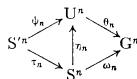
\includegraphics[keepaspectratio]{images/part001_756df219.jpg}}

where each arrow represents a vector space isomorphism. If \(x_{1}, x_{2}, \ldots, x_{n}\) are in \(g\) , \(\eta_{n}\) maps the product \(x_{1}x_{2}\ldots x_{n}\) , calculated in S, to the element

\[
\frac {1}{n !} \sum_ {\sigma \in \mathfrak {S} _ {n}} x _ {\sigma (1)} x _ {\sigma (2)} \dots x _ {\sigma (n)}
\]

calculated in U.

COROLLARY 5. Let \(\mathfrak{h}\) be a subalgebra of the Lie algebra \(\mathfrak{g}\) and \(\mathrm{U}'\) its enveloping algebra. Suppose that the K-modules \(\mathfrak{h}\) and \(\mathfrak{g} / \mathfrak{h}\) are free (for example if \(\mathrm{K}\) is a field). Let \((x_{\alpha})_{\alpha \in \mathbb{L}}\) be a basis of \(\mathfrak{h}\) and \((y_{\beta})_{\beta \in \mathbb{M}}\) a family of elements of \(\mathfrak{g}\) whose canonical images in \(\mathfrak{g} / \mathfrak{h}\) form a basis of \(\mathfrak{g} / \mathfrak{h}\) .

\begin{enumerate}
\def\labelenumi{(\alph{enumi})}
\item
  The canonical homomorphism of \(\mathbf{U}'\) into \(\mathbf{U}\) is injective.
\item
  If \(\mathbf{M}\) is totally ordered, the elements \(y_{\beta_1} \ldots y_{\beta_q}\) , where \(\beta_1 \leqslant \cdots \leqslant \beta_q\) , form a basis of \(\mathbf{U}\) considered as a left or right module over \(\mathbf{U}'\) .
\end{enumerate}

We give \(L \cup M\) a total ordering such that every element of L is less than every element of M. The elements \(x_{\alpha_{1}}x_{\alpha_{2}}\ldots x_{\alpha_{p}}\) calculated in \(U'\) (where \(\alpha_{1} \leqslant \cdots \leqslant \alpha_{p}\) ) form a basis of \(U'\) (Corollary 3). The elements

\[
x _ {\alpha_ {1}} \dots x _ {\alpha_ {p}} y _ {\beta_ {1}} \dots y _ {\beta_ {q}}
\]

calculated in U (where \(\alpha_{1} \leqslant \cdots \leqslant \alpha_{p} \leqslant \beta_{1} \leqslant \cdots \leqslant \beta_{q}\) ) similarly form a basis of U. Hence the canonical homomorphism of U' into U maps the elements of a basis of U' to linearly independent elements of U and is therefore injective. It is moreover seen that the \(y_{\beta_1} \ldots y_{\beta_q}\) (where \(\beta_{1} \leqslant \cdots \leqslant \beta_{q}\) ) form a basis of U considered as a left U'-module. Ordering L ∪ M so that every element of M is less than every element of L, it is similarly seen that the \(y_{\beta_1} \ldots y_{\beta_q}\) (where \(\beta_{1} \leqslant \cdots \leqslant \beta_{q}\) ) form a basis of U considered as a right U'-module.

Under the conditions of Corollary 5, U' is identified with the subalgebra of U generated by h by means of the canonical homomorphism of U' into U.

COROLLARY 6. Suppose that the K-module g is the direct sum of subalgebras \(g_{1}, g_{2}, \ldots, g_{n}\) and that each \(g_{i}\) is a free K-module. Let \(U_{i}\) be the enveloping algebra of \(g_{i}\) ( \(1 \leqslant i \leqslant n\) ). Let \(\phi\) be the K-linear mapping of the K-module \(U_{1} \otimes_{K} \cdots \otimes_{K} U_{n}\) into U defined by the multilinear mapping ( \(u_{1}, \ldots, u_{n}\) ) \(\mapsto u_{1} \ldots u_{n}\) of \(U_{1} \times \cdots \times U_{n}\) into U. Then \(\phi\) is a K-module isomorphism.

Let \((x_{\lambda}^{i})_{\lambda \in L_{i}}\) be a basis of \(g_{i}\) . We totally order \(L_{1} \cup \cdots \cup L_{n}\) so that every element of \(L_{i}\) exceeds every element of \(L_{j}\) for \(i \geqslant j\) . Then the elements:

\[
\left(x _ {\lambda_ {1}} ^ {1} x _ {\lambda_ {2}} ^ {1} \dots x _ {\lambda_ {p}} ^ {1}\right) \otimes \dots \otimes \left(x _ {\nu _ {1}} ^ {n} x _ {\nu _ {2}} ^ {n} \dots x _ {\nu _ {q}} ^ {n}\right),
\]

where \(\lambda_{1}\leqslant\lambda_{2}\leqslant\cdots\leqslant\lambda_{p}\leqslant\cdots\leqslant\nu_{1}\leqslant\nu_{2}\leqslant\cdots\leqslant\nu_{q}\) , constitute a basis of \(U_{1}\otimes_{K}\cdots\otimes_{K}U_{n}\) . They are mapped by \(\phi\) to the elements:

\[
x _ {\lambda_ {1}} ^ {1} x _ {\lambda_ {2}} ^ {1} \dots x _ {\lambda_ {p}} ^ {1} \dots x _ {\nu_ {1}} ^ {n} x _ {\nu_ {2}} ^ {n} \dots x _ {\nu_ {q}} ^ {n}
\]

which constitute a basis of U. Hence the corollary.

COROLLARY 7. If K is an integral domain and g is a free K-module, the algebra U has no divisors of zero.

G is isomorphic to a polynomial algebra over K (Theorem 1) and is therefore an integral domain (Algebra, Chapter IV, § 1, no. 4, Theorem 1). Hence the corollary (Commutative Algebra, Chapter III, § 2, no. 3, Proposition 1).

